%# -*- coding: utf-8-unix -*-
%%==================================================
%% chapter01.tex for SJTU Master Thesis
%%==================================================

%\bibliographystyle{sjtu2}%[此处用于每章都生产参考文献]
\chapter{混合存储系统介绍}
\label{chap:hss_intro}

\section{混合存储系统的基本概念}

混合存储系统是指利用多种不同的存储设备构建的一套数据存储系统。混合存储系统之所以存在的根本原因在于存储设备的读写性能与成本成正相关。最理想的存储系统应该是讲所有的数据都存储在最高速的存储设备中,这样存储系统的性能能达到最高,但是由于同样成本下高速设备的存储容量至少要比低速设备小一个量级,因此这样的系统的成本对于一般用户而言难以接受。而混合存储系统能充分利用不同存储设备的特性,将绝大部分用户的数据存储在低速设备中,而只将用户会频繁使用的数据放在高速设备中以提供对这些数据的高存取性能,使得系统整体对外表现为大容量、高性能、高性价比。

\section{主流的存储设备的特性}

\subsection{磁盘}

磁盘,即机械磁盘,又被称为硬盘,是应用最广泛的一种存储设备。磁盘通过离磁盘片很近的磁头的电流改变磁盘片上存储的极性的方式来存储数据,数据的读取则通过与存储相反的方式进行。磁盘依照接口的不同可大致分为ATA、SATA、SCSI及SAS四种,常见的转速为每分钟4200转到每分钟10000转,工业级的高档磁盘的转速能达到每分钟15000转。磁盘的顺序读写性能与随机读写性能差异巨大,顺序读写时数据的传输速率能达到200MB/s,但随机读写时IOPS(I/O per second,即每秒的I/O操作)仅为约75,这是由于磁盘的磁头的机械移动所带来的限制,而磁盘的容量则依照摩尔定律稳步增长,因此磁盘的容量与性能的矛盾日趋严重。总的来看磁盘具有大容量、低成本、适合顺序读写的特点。

\subsection{固态盘}

固态盘(SSD:solid state disk)是使用固态电子存储芯片阵列而制成的硬盘,由控制单元和存储单元(FLASH芯片、DRAM芯片)组成。SSD对存储介质的组织类似树状结构,图\ref{fig:ssd_phy}所示为三星的4GB闪存的内部组织结构\cite{agrawal2008design}。一个4GB的package由2个die(也被称为chip即芯片)组成,每个die由4个plane组成,每个plane由2048个block组成,每个block由64个4KB大小的page组成。对于不同die的操作可以并行执行,对每个die的操作最后落到1个或2个plane执行,当操作落到2个plane时,只能是plane0及plane1或plane2及plane3,而不能交叉。SSD由于不像磁盘有磁头的机械移动,而都是通过电子信号的方式,所以与磁盘相比具有体积小、质量小、能耗低、访问延迟小的特点\cite{agrawal2008design, dirik2009performance},尤其在随机读写方面比磁盘高出一个量级。虽然近年来随着工艺的进步,SSD的容量日趋提高、成本日趋下降,但与磁盘相比仍显成本高容量小,并且由于SSD有写前擦除的次数限制,耐用性方面不如磁盘,因而SSD仍未完全取代磁盘。

\begin{figure}[!htp]
  \centering
  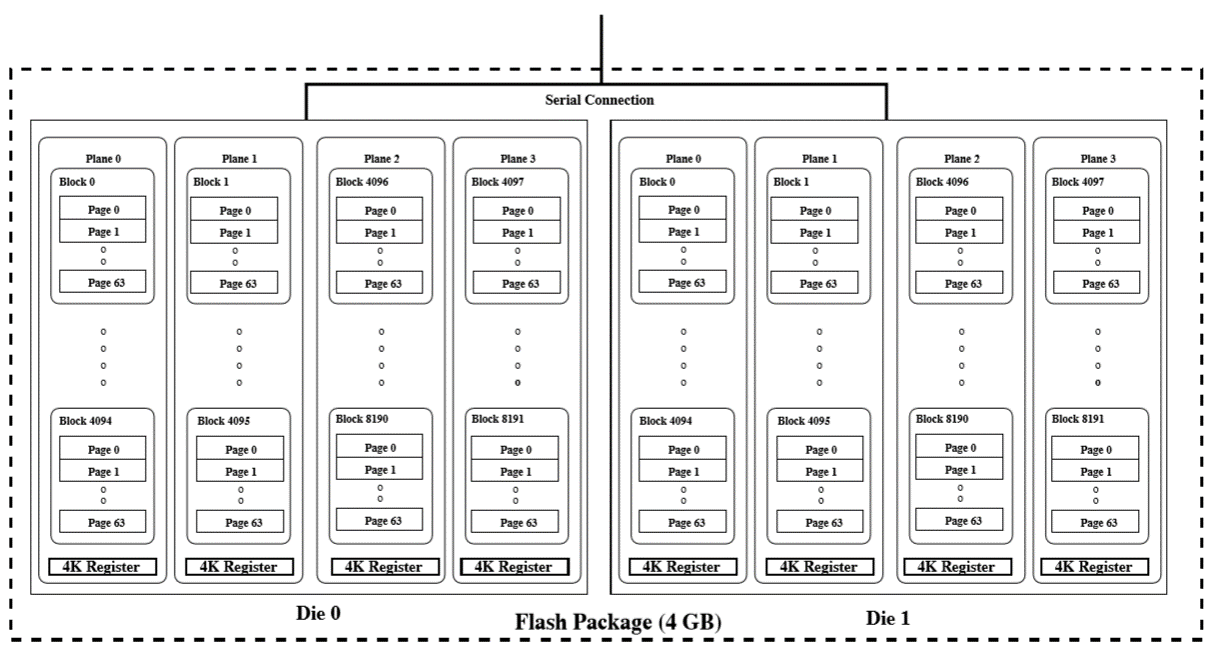
\includegraphics[width=\textwidth]{ssd_phy.png}
  \hspace{1cm}
  \bicaption[fig:ssd_phy]{固态盘存储介质的组织}{固态盘存储介质的组织}{Fig}{organization of solid state disk storage media}
\end{figure}

\subsection{非易失性随机存储器}

非易失性随机存储器(NVRAM:Non-Volatile Random Access Memor)是指断点后仍能保持数据的一种随机访问存储器。早期的NVRAM由RAM加上电池组成,而近年来新型NVRAM已不需要电池。与SSD相比,NVRAM不存在写前擦除的操作,因此写操作比SSD更快且没有因写前擦除的次数限制带来的耐用性问题,但是与SSD相比,NVRAM的容量更小、成本更高,因此常用来作为缓存设备,而不作为主存储设备使用。

\subsection{主流的存储设备的对比}

以性能、成本、容量为三大指标,磁盘、SSD、NVRAM的对比如表\ref{tab:hdd_ssd_nvram}所示。可以看到,NVRAM、SSD、HDD的性能分别为ns级、μs级(写操作为ms级)、ms级,容易分别为MB级、GB级、TB级,成本为$10^{3}$级、$10^{0}$级、$10^{-1}$级。可见不同的存储设备各有各的优势与劣势,要选取单一种类的存储设备来构建一个同时满足高性能、高容量、低成本的存储系统是极其困难的,而将不同存储设备组合起来构建混合存储设备则有可能让这些存储设备形成互补。

\begin{table}[!hpb]
    \centering
    \bicaption[tab:hdd_ssd_nvram]{磁盘、SSD、NVRAM的对比}{磁盘、SSD、NVRAM的对比}{Table}{differences among HDD, SSD and NVRAM}
    \begin{tabular}{cccccc} \toprule
      存储设备 & 读延迟 & 写延迟 & 写前擦除延迟 & 容量量级 & \$/GB \\ \midrule
      NVRAM(FRAM) & 55ns & 55ns & N/A & $10^{0}$MB & $4 \times 10^{3}$ \\
      NVRAM(BBDRAM) & 70-100ns & 70-100ns & N/A & $10^{0}$GB & $2 \times 10^{3}$ \\
      SSD(基于闪存) & 25μs & 200μs & 1.5ms & $10^{2}$GB & $1 \times 10^{0}$ \\
      HDD(SATA接口) & 8.5ms & 9.5ms & N/A & $10^{3}$GB & $1 \times 10^{-1}$ \\ \bottomrule
    \end{tabular}
  \end{table}

\section{混合存储系统的发展历程}

\subsection{基于NVRAM与HDD的混合存储系统}

传统上,将RAM作为HDD的缓存一直是提高存储系统整体性能的重要手段\cite{belady1966study},系统将用户频繁访问的数据放在RAM中,当访问该数据时直接从RAM中获取数据而非从HDD中获取数据,使系统对外表现为RAM的性能。然而使用RAM作为HDD的缓存只能提高系统整体的读性能,而对写性能的提升有限,这并非是由于RAM的容量相较HDD的容量太小导致缓存的容量不够用,而是由于如果发生断电,那么RAM上的数据就会丢失,而RAM作为HDD的缓存,上面可能会保有经过修改而尚未写回到HDD的脏数据,如果发生断点,那么这些数据的修改就会丢失,所以为了保证数据的可靠性,需要将RAM上的脏数据写回到HDD上,这就导致系统面临提升写性能与保障数据可靠性的两难境地。同时脏数据在RAM中驻留的时间越长,那么它再次受到改写的概率与断点带来的损失也越大,因此一般都会限制脏数据在RAM中的驻留时间,最终导致系统整体的写性能提升不显著。

NVRAM作为非易失性随机存储器,给把RAM作为HDD缓存的系统带来了新的可能。将所有的脏数据都存放在NVRAM上\cite{baker1992non},而普通数据放在NVRAM或RAM上就可以保证即使断点,数据的修改仍然能被保留,使得系统不需要频繁地将数据写回到HDD中以保证数据的可靠性,提升了系统整体的写性能。另一种作法是将NVRAM作为日志记录设备,将写操作以追加日志的形式写入NVRAM中,当NVRAM的容量使用到一定程度后再一次写回到HDD中,这样即使发生断点,系统也能从NVRAM的日志中重建出最新的数据。

总体而言,基于NVRAM与HDD的混合存储系统对于系统的可靠性问题有了比较好的解决,但对于系统整体的性能提高仍然有限。原因在于在较早的时候,NVRAM的容量且成本高,这使得将NVRAM作为缓存,缓存容量有限,对系统的性能提高有限。而现在虽然NVRAM的容量在不断增长,大的NVRAM甚至能达到8GB的容量,但是与HDD的容量增长相比仍然有限,NVRAM与HDD的容量比仍在不断缩小,导致缓存的命中率不断下降,系统的性能提升的效果也在不断降低。

\subsection{基于不同转速的HDD的混合存储系统}

在20世纪90年代,产业界一度热衷于研究将不同规格不同转速的HDD组合构建混合存储系统,其基本思想也是基于将数据区分为冷热数据的想法,将用户需要经常访问的热数据放在高转速的磁盘上,而将用户不经常访问的冷数据放在低转速的磁盘上。但由于磁盘的性能瓶颈出在磁头的机械移动上,而不同转速的磁盘的磁头的机械移动并不存在显著差异,因此不同转速的磁盘构建的混合存储系统的随机读写性能并没有显著的提升。

\subsection{基于SSD与HDD的混合存储系统}

近年来,SSD的快速发展以及SSD与HDD良好的互补性,使得基于SSD与HDD的混合存储系统的研究成为存储领域的一个重要研究方向。产业界尤其表现出浓厚的兴趣,IBM\cite{ibm2010ds8000}、NetApp\cite{netapp}、EMC\cite{laliberte2009automate}等企业已经生产出了一些采用了或者支持基于SSD与HDD的混合存储的产品。

对目前已有的基于SSD与HDD的混合存储系统的研究发现SSD的写前擦除特性与擦除次数限制对系统整体的写性能影响很大,系统如果频繁地将数据写入SSD就会导致SSD的寿命减少,降低系统的可靠性,但如果频繁地将数据写入HDD则会导致系统的写性能下降,SSD无法发挥出其优势。针对这一问题,有的研究着眼于对于SSD磨损均衡的改良\cite{王增辉2015磨损均衡在提高, 李恒恒2016基于, 陈晓敏2010基于},有的研究着眼于数据冷热识别算法的研究\cite{刘庆宾2016面向多用户的, 闫林2014基于},将真正需要的数据放在SSD中。

\section{本章小结}

本章主要介绍了混合存储系统的基本概念,然后介绍了目前主流的存储设备的特性,并对比分析了这些主流存储设备在性能、容量、成本方面的差异。最后对混合存储系统的发展历程做了简单的介绍,对发展中不同混合存储系统的优劣进行了简单的阐述。对于这些混合存储系统的优劣将引出在下一章中要介绍的混合存储系统中的关键技术。